\section{Piezoelektrizität}
Die Piezoelektrizität ist per Definition spannend.
Sie beschreibt die Eigenschaft, dass gewisse Kristalle eine elektrische Spannung erzeugen, wenn machanischer Druck auf sie ausgeübt wird.

\begin{figure}
    \centering
    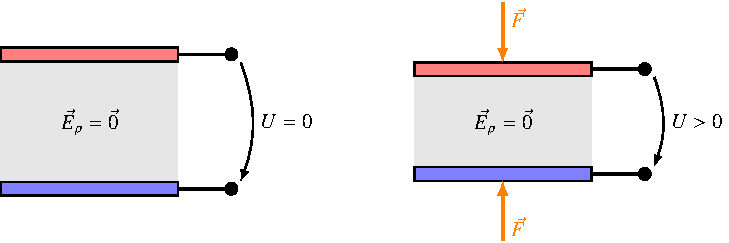
\includegraphics[]{papers/punktgruppen/figures/piezo} %das Efeld mit Naoki disskutieren, müssen sicher gehen, dass es mit jenen in Abbildung Piezo aufbau übereinstimmt
    \caption{Piezoelektrisches Material in Ruhe und unter Druck}
    \label{fig:punktgruppen:basicPiezo}
\end{figure}

\subsection{Polarisierung}
Piezoelektrizität basiert darauf, dass zwischen den Oberflächen des Kristalles ein Ladungsungleichgewicht entsteht siehe Abbildung\ref{fig:punktgruppen:basicPiezo}.
Dieses Ungleichgewicht resultiert, 
weil durch den mechanischen Druck auf der einen Oberfläche des Kristalles positiv Ione näher an die Oberfläche gelangen,
wärend auf der gegenüberliegenden Oberfläche sich mehr negative Ionen Sammeln.
Das sich die atomare Struktur eines Kristalles unter Druck genau so verformt ist nicht bei jedem Kristall gegeben.
Der Aufbau und somit auch die Symmetrie des Kristalles sind daher relevant für die Entstehung dieses Effektes.

\begin{figure}
    \centering
    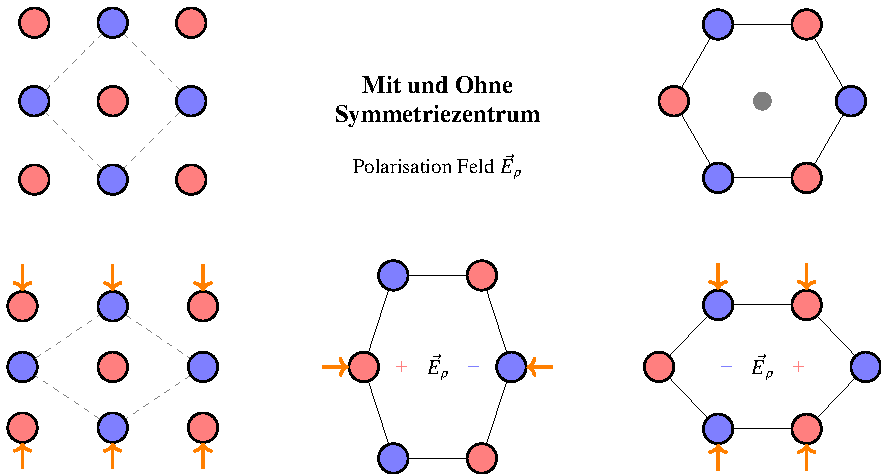
\includegraphics[]{papers/punktgruppen/figures/piezo-atoms} 
    \caption{
        Kristallstrukturen mit und ohne piezoelektrischer Eigenschaft.
        \texttt{TODO: adapt figure for paper with subfigure markers.}
    }
    \label{fig:punktgruppen:atomPiezo}
\end{figure}

\subsection{Atomarer Aufbau}
Die Polarisation resultiert über eine gesamte Oberfläche eines Kristalles, entscheidend ist aber der atomare Aufbau.
Wir wollen dazu die verschiedenen Kristallstrukturen auf Abbildung \ref{fig:punktgruppen:atomPiezo} diskutieren.
In Abbildung \ref{fig:punktgruppen:atomPiezo} gilt für alle Strukturen, dass rote Kreise Positive Ionen und blaue negative Ionen repräsentieren. 
%liste oder anderes format?..
Struktur$(a)$ zeigt ein piezoelektrisches Material in Ruhe. Struktur $(b)$ ist dasselbe Kristallgitter, jedoch wird es senkrecht belastet. 
Eingezeichnet ist auch das elektrische Feld, welches entsteht, weil mitlleren Ladungsträger weiter auseinander gerdrückt werden.
Als hilfe zur Vorstellung kann man $(b)$ zwischen zwei leitende Platten setzen, 
so wird ersichtlich, dass mit wachsendem Druck eine negative Ladung an die rechte Platte gedrückt wird,
während sich die positiven Ionen weiter entfernen. 
$(d)$ ist nicht piezoelektrisch.
Dies wird ersichtlich, wenn man $(d)$ unterdruck setzt und sich die Struktur zu $(e)$ verformt.
Setzt man  $(e)$ gedanklich auch zwischen zwei leitende Platten scheint es als würden rechts mehr Positive Ionen in die Platte gedrückt werden 
und links umgekehrt.
Dies ist aber nicht mehr der Fall, wenn der Kristall nach oben und periodisch wiederholt.
Struktur $(c)$ zeigt $(a)$ in unter horizontaler Belastung. 
Was in zwischen $(b)$ und $(c)$ zu beobachten ist, ist dass das entstandene Ladungsdifferenz orthogonal zu der angelegten Kraft entsteht,
im Gegensatz zu $(b)$.
Daraus kann man schlissen, dass $(a)$ keine Rotationssymmetrie von $90^\circ$ besitzen kann, weil die Eigenschaften ändern bei einer $90^\circ$ Drehung. 
Das Fehlen dieser Rotationssymmetrie kann mit betrachten von $(a)$ bestätigt werden. 

\subsection{Punktsymmetrie}\footnote{In der Literatur wird ein Punktsymmetrisches Kristallgitter oft als Kristallgitter mit Inversionszentrum bezeichnet.}
Piezoelektrische Kristalle können nicht Punktsymmetrisch sein.
Kristallgitter, bei welchen eine Punktspiegelung eine symmetrische Operation ist, können keine piezoelektrische Kristalle bilden.
Auf Abbildung \ref{fig:punktgruppen:atomPiezo} ist bewusst $(a)$ ein nicht Punktsymmetrischer Kristall mit einem Punktsymmetrischen $(d)$ verglichen worden.
Als vereinfachte Erklärung kann mann sich wieder das Bild vor augen führen, eines Kristalles, 
welcher unter Druck auf der einen Seite negative und der anderen Seite positive Ionen an seine Oberfläche verdrängt.
Spiegelt man nun den Kristall um den Gitterpunkt in der mitte des Kristalles, so würden die negativen Ionen auf den Positiven auf der anderen seite landen,
was der Definition einer Symmetrie deutlich widerspricht.

\subsection{Vom Kristall zum Feuer}
Piezoelektrizität hat durchaus nutzen im Alltag.
Feuerzeuge welche nicht auf dem Prinzip beruhen einen Zündstein abzuschleifen, 
sonder ohne Verschleiss auf Knopfdruck einen Zündfunken erzeugen, basieren auf dem Prinzip der Piezoelektrizität.
Drückt der Nutzende auf den Zündknopf spannt sich eine Feder bis zu einer Konfigurierten Spannung.
Wird vom Nutzenden weiter gedrückt entspannt sich die Feder schlagartig und beschleunigt mit der gespeicherten Energie ein Hammer,
welcher auf das Piezoelement aufschlägt.
Der augenblicklich hohe Druck sorgt an den Piezokontakten für eine eben so Kurze aber hohe elekrische Spannung.
Die Spannung reicht aus, um eine Funkenstrecke zu überwinden und so eine entflammbares Gas zu entzünden.
Sollten Sie also eines Tages in die Situation geraten, in welcher Sie zwei verschiedene Kristalle vor sich haben
und ein piezoelektrisches Feuerzeug bauen müssen,
wobei Sie aber wissen, dass einer eine Punktsymmetrie aufweist,
versuche sie es mit dem anderen.
Ich muss aber anmerken, dass aus den $21$ möglichen Kristallsymmetrien ohne Punktsymmetrie einer nicht piezoelektrisch ist.
ein wenig glück brauchen Sie also immer noch.
